\chapter{Theoretische Grundlagen}
\label{chap:two}
In diesem Kapitel werden die theoretischen Grundlagen für die weiteren Kapitel gelegt. In einem
ersten Abschnitt werden Grundlagen der bibliothekarischen Statistik im Zusammenhang mit Budgetplanung
und Mittelallokation erläutert. Im darauffolgendem Abschnitt geht es um Datenvisualisierungen und deren Einsatz
für die Datenpräsentation. Abschließend wird Business-Intelligence-Software eingeführt als Schmelzpunkt der 
beiden vorangegangen Kapitel.

\section{Bibliothek und Statistik}
\label{chap:two_one}
Die Etatplanungen von Bibliotheken richten sich nach deren Informations- und Versorgungsauftrag. 
Seit Beginn der 1990er Jahre kämpfen Bibliotheken mit der größer werdenden Informationsflut, den steigenden Preisen, 
zunehmenden Kommerzialisierungstendenzen in der Verlagslandschaft und neuen Medientypen. 
Zu nennen wären hier konkret: die Explosion der Zeitschriftenpreise im Bereich der \acrfull{STM},
das Aufkommen von E-Publishing und die Konzentration auf wenige Verlage. Demgegenüber steigen Bibliotheksetats nur mäßig und
damit ein Kaufkraftverlust. \cite[161]{moravetz-kuhlmann_monika_erwerbungspolitik_2015}

Diese Tendenzen betrafen nicht nur die Universitätsbibliotheken, sondern auch Spezialbibliotheken von Forschungseinrichtungen.
Gegen diese Entwicklung haben Bibliotheken Instrumente entwickelt, die versuchen den Informationsauftrag trotz der Widrigkeiten zu erfüllen.
Es entstanden von Bund und Ländern geförderte Konsortien, um den Kostendruck auf Bibliotheken, insbesondere im Bereich der elektronischen
Fachinformationen, zu mildern. Neue Geschäftsmodelle sollten dies bezüglich entwickelt werden, 
um Preisnachlässe bei den elektronischen Informationsressourcem zu erzielen. 
\cite[169 ff.]{moravetz-kuhlmann_monika_erwerbungspolitik_2015}. So konnte das Projekt Deal in den letzten Jahren 
verschiedene Abschlüsse mit großen Verlagen zum Abschluss bringen. (Quelle)



Um den Veränderungen lokal zu begegnen, ist es wichtig, das Bibliotheksbudget kosteneffizient zu planen. 
Dies geschieht in größeren Bibliotheken durch Etatbedarfs- und Etatverteilungsmodelle. 
Ziel dieser Modelle ist die transparente und gerechte Verteilung knapper Ressourcen innerhalb der Bibliothek. 

Grundlage auf denen diese Modelle basieren sind statistische Daten. Was sind statistische Daten? Diese Daten werden durch Evaluationsverfahren erhoben. 
Im bibliothekarischen Kontext sind die sammlungs-, nutzungsbezogene und die nutzerbezogene Evaluation zu finden.  
Die sammlungsbezogene Evalution betrifft den Bestand, dessen Größe und Wachstum über die Jahre.

Nutzungsbezogene Evalution betrifft die Lesesaalnutzung, die Ausleihe vor-Ort, die Nutzung des Fernleihservices oder Dolumentlieferdienste 
und die Online-Nutzung. Ziele dabei sind die Identifizierung von ausleihträchtigen Medienbeständen (Vormerkungs- und Rennerlisten), 
die Deacquisition schlecht oder gar nicht genutzter Titel. Ebenso kann die Evaluation von Fernleih- und Dokumentenlieferungen Hinweise auf Bestandslücken liefern. 
\cite[255 ff.]{johannsen_jochen_bestands-_2015}. Die nutzerbezogene Evaluation ist zentriert um den Nutzer und dessen Informitionsbedürfnisse.
Fundamental ist der Unterschied zwischen den einzelnen Evaulationsverfahren in der Erhebung der Daten. 
Die sammlungs- und nutzungsorientierten Evaluationsverfahren basieren auf der Erhebung von quantitativen Daten wie Bestandsgröße oder der Anzahl von Ausleihen nach Titel. 
Während nutzerbezogene Evaluation qualitative Daten aus zum Beispiel Befragungen erhebt. \cite[461 ff.]{blake_data_2004}
Statistriken sind wichtig…

Im deutschen Bibliothekswesen gab es den Bibliotheksindex (BIX), der ursprünglich 
für die Leistungsmessung in Öffentlichen Bibliotheken konzipiert wurde. 
2002 wurde er erweitert auf Wissenschaftliche Bibliotheken. 2015 wurde der BIX aufgrund von Finanzierungsproblemen eingestellt. 
Daneben gibt es seit 1974 die umfangreiche Deutsche Bibliotheksstatistik (DBS). 
Träger der DBS sind das hbz, Kompetenznetzwerk für Bibliotheken (KBN), KMK sowie die Bibliotheken
Aufgabe dieser ist die jährliche Erhebung der Statistikdaten von Kennzahlen von Bibliotheken. 
Seit 1999 werden die Daten nur noch online erfasst, ausgewertet und präsentiert. 
(https://www.egms.de/static/en/journals/mbi/2008-8/mbi000102.shtml)
Neben den Gesamtauswertungen der DBS, einer Bibliothekssuchmachine für Öffentliche Bibliotheken, 
bietet sie eine variable Auswertung nach individuellen Abfragen der DBS-Daten. 
Dennoch bietet die DBS vielmehr eine Datengrundlage für die Auswertung der Daten an.



\clearpage
Bibliotheksrahmen - Etatplanung - Etatbedarfe, Zielsetzung der Bibliothek\\
Begriffe wie Mittelallokation\\
Bestandsmanagement\\
Was ist Statistik\\
Erhebung von qualitativen und quantitativen Daten Bsp.:\\
Konzentration auf quantitative Daten wie ...\\
hat schon immer große Rolle in Bibliotheken gespielt\\
BIX, Deutsche Bibliotheksstatistik (seit wann)\\
Warum ist Messbarkeit von bibliothekarischen Daten wichtig?\\
Welchen Impact für Budgetplanung können statistische Daten haben?\\
Was können statistische Daten in Bibliotheken aussagen?\\
Welche Daten werden in Bibliotheken erhoben\\
Sammlungsbezogene Evaluierung
Nutzerbezogene Evaluation\\
Nutzungsbezogene Evaluation\\
quantitativ und qualitativ:\\
Counter-Statistiken \& Standards\\

\clearpage

\section{Datenvisualisierung}
Mit den Siegeszug des Computers in den 1980/90er Jahren sind \dots\\
Was ist unter Datenvisualisierung zu verstehen?\\
leicht verschiedene Begriffsdefinitionen
Vielzahl von Begriffen\\ 
Oberbegriff für Informationsvisualisierung / Scientific Visualization\\
Abgrenzung zu Infographics\\
Zu welchem Zweck\\
Eigenschaften\\
Wie Datenvisualisierungen gestaltet werden sollen - simpel\\
Grundlage - Daten - quantitativ / qualitativ
Warum Datenvisualisierung wichtig ist?\\
Was erzählen Datenvisualisierungen mehr als Zahlenkolonnen?\\
Perception of the eye - schnellere Auffassung
Welche Datenvisualisierungen gibt es?\\
Wo kommen Daternvisualisierungen zum Einsatz?\\



% \begin{figure}[ht]
%     \centering
%         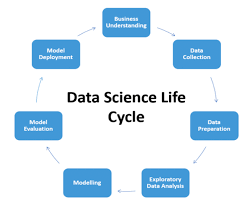
\includegraphics[width=8cm]{ds_cycle}
%         \caption{Data Science Cycle}
%         \label{fig:data science}
% \end{figure}



\clearpage
\section{Business-Intelligence-Systeme}

Was sind Business-Intelligence-Löungen?\\
%Wo kommen Buisiness-Intelligence-Lösungen zum Einsatz zum Einsatz?
Es gibt eine Vielzahl kommerzieller Lösungen für den Bibliotheksbereich, die auf Business-Intelligence-Software basieren.
Zu nennen wären \textit{AlmaAnalytics} für das Next-Generation-Library-System \textit{Alma} von \textit{ExLibris}\footnote{\url{https://www.exlibrisgroup.com/products/alma-library-services-platform/alma-analytics}
Stand: 26.05.2020}, \textit{BibControl} von \textit{OCLC}\footnote{\url{https://www.oclc.org/de/bibcontrol.html} Stand: 26.05.2020},
\textit{CollectionHq} von \textit{Baker \& Taylor}\footnote{\url{https://www.collectionhq.com/} Stand: 26.05.2020} oder \textit{Libinsight} von \textit{SpringShare}\footnote{\url{https://springshare.com/libinsight/} Stand: 26.05.2020}.
Darüber hinaus gibt es Business-Intelligence-Applikationen, die von
Bibliotheken für Reporting, Datenanalyse und Datenvisualisierung adaptiert werden,
wie zum Beispiel \textit{Tableau} von der Firma \textit{Tableau Software} oder
\textit{Crystal Reports} von \textit{SAP}.
Diese Applikationen sind entweder
an bestimmte Bibliothekssysteme zurückgebunden, limitiert in ihren
Funktionen\cite{golas_statistische_2018} oder zu generisch.
Überdies wird sowohl von \textit{HeBis} bzw. von der
Lokal-Bibliothekssystembetreuung als auch von der \textit{mpdl} keine Applikation
in dieser Richtung angeboten.
Ebenso ist ungewiss, wann die Ablösung des schon betagten \textit{CBS/LBS} hin zu
einem neuen Next-Generation-Library-System im \textit{HeBis-Verbund} stattfinden wird und ob
es ein Modul zur statistischen Datenerhebung liefern wird.
